\documentclass[margin=3cm,mikulas,portrait,final]{myposter}
%\documentclass[a4shrink,portrait,final]{baposter}
% Usa a4shrink for an a4 sized paper.

\tracingstats=2

\usepackage{times}
\usepackage{calc}
\usepackage[intlimits]{amsmath}
\usepackage{amssymb}
\usepackage{relsize}
\usepackage{multirow}
\usepackage{bm}
\usepackage{ulem} % colored underlining, strike out

\usepackage[czech]{babel}
\usepackage[utf8]{inputenc}

\usepackage{graphicx}
\usepackage{multicol}
%\usepackage{wasysym}


\usepackage{nicefrac}
\usetikzlibrary{positioning,calc,arrows,snakes,backgrounds,patterns,shapes,fit,shadows,plotmarks}

\usepackage{pgfbaselayers}
\pgfdeclarelayer{background}
\pgfdeclarelayer{midground}
\pgfdeclarelayer{foreground}
\pgfsetlayers{background,midground,main,foreground}

\usepackage{helvet}
%\usepackage{bookman}
\usepackage{palatino}

\selectcolormodel{cmyk}

%%%%%%%%%%%%%%%%%%%%%%%%%%%%%%%%%%%%%%%%%%%%%%%%%%%%%%%%%%%%%%%%%%%%%%%%%%%%%%%%
% Picture inclusion settings.
%%%%%%%%%%%%%%%%%%%%%%%%%%%%%%%%%%%%%%%%%%%%%%%%%%%%%%%%%%%%%%%%%%%%%%%%%%%%%%%%
\newcommand{\captionfont}{\footnotesize}
\graphicspath{{obr/}}

%%%%%%%%%%%%%%%%%%%%%%%%%%%%%%%%%%%%%%%%%%%%%%%%%%%%%%%%%%%%%%%%%%%%%%%%%%%%%%%%
% Custom math commands.
%%%%%%%%%%%%%%%%%%%%%%%%%%%%%%%%%%%%%%%%%%%%%%%%%%%%%%%%%%%%%%%%%%%%%%%%%%%%%%%%
\newcommand{\flx}{\varphi}
\newcommand{\bx}{\mathbf{x}}
\newcommand{\bomega}{\mathbf{\Omega}}
\renewcommand{\it}[1]{^{#1}}
\newcommand{\pd}[3][]{\frac{\partial^{#1}#2}{\partial#3^{#1}}}
\newcommand{\imply}{\Rightarrow}
\newcommand{\oper}[1]{\mathcal{#1}}
\renewcommand{\div}{\nabla\cdot}
\newcommand{\grad}{\nabla}
\newcommand{\bF}{\mathbf{F}}
\newcommand{\bY}{\mathbf{Y}}
\newcommand{\bJ}{\mathbf{J}}
\newcommand{\bO}{\mathbf{0}}
\newcommand{\lightout}[1]{\textcolor{Gray}{\itshape #1}}
\newcommand{\plus}{(+)}
\newcommand{\minus}{(--)}
\newcommand{\vint}[1]{\int\nolimits_V#1\,\mathrm{d}{V}}
\newcommand{\vvec}[2]{\begin{bmatrix} #1\\#2 \end{bmatrix}} 
\newcommand{\dt}{\Delta t}
\newcommand{\testT}{\Theta_j}
\newcommand{\testN}{\Phi_i}
\newcommand*{\norm}[1]{\mathopen\Vert #1 \mathclose\Vert}
\newcommand{\Muline}{\bgroup\markoverwith
{\textcolor{colM}{\rule[-0.5ex]{2pt}{0.4pt}}}\ULon}
\newcommand{\blueuline}{\bgroup\markoverwith
{\textcolor{Blue}{\rule[-0.5ex]{2pt}{0.4pt}}}\ULon}


%%%%%%%%%%%%%%%%%%%%%%%%%%%%%%%%%%%%%%%%%%%%%%%%%%%%%%%%%%%%%%%%%%%%%%%%%%%%%%%%
% Multicol settings
%%%%%%%%%%%%%%%%%%%%%%%%%%%%%%%%%%%%%%%%%%%%%%%%%%%%%%%%%%%%%%%%%%%%%%%%%%%%%%%%
\setlength{\columnsep}{0.7em}
\setlength{\columnseprule}{0mm}


%%%%%%%%%%%%%%%%%%%%%%%%%%%%%%%%%%%%%%%%%%%%%%%%%%%%%%%%%%%%%%%%%%%%%%%%%%%%%%%%
% Save space in lists. Use this after the opening of the list
%%%%%%%%%%%%%%%%%%%%%%%%%%%%%%%%%%%%%%%%%%%%%%%%%%%%%%%%%%%%%%%%%%%%%%%%%%%%%%%%
\newcommand{\compresslist}{%
\setlength{\itemsep}{1pt}%
\setlength{\parskip}{0pt}%
\setlength{\parsep}{0pt}%
}


%%%%%%%%%%%%%%%%%%%%%%%%%%%%%%%%%%%%%%%%%%%%%%%%%%%%%%%%%%%%%%%%%%%%%%%%%%%%%%
%%% Begin of Document
%%%%%%%%%%%%%%%%%%%%%%%%%%%%%%%%%%%%%%%%%%%%%%%%%%%%%%%%%%%%%%%%%%%%%%%%%%%%%%

\begin{document}
\pagestyle{empty}
%%%%%%%%%%%%%%%%%%%%%%%%%%%%%%%%%%%%%%%%%%%%%%%%%%%%%%%%%%%%%%%%%%%%%%%%%%%%%%
%%% Here starts the poster
%%%---------------------------------------------------------------------------
%%% Format it to your taste with the options
%%%%%%%%%%%%%%%%%%%%%%%%%%%%%%%%%%%%%%%%%%%%%%%%%%%%%%%%%%%%%%%%%%%%%%%%%%%%%%
% Define some colors
\definecolor{silver}{cmyk}{0,0,0,0.3}
\definecolor{yellow}{cmyk}{0,0,0.9,0.0}
\definecolor{reddishyellow}{cmyk}{0,0.22,1.0,0.0}
\definecolor{black}{cmyk}{0,0,0.0,1.0}
\definecolor{darkYellow}{cmyk}{0,0,1.0,0.5}
\definecolor{darkSilver}{cmyk}{0,0,0,0.1}

\definecolor{lightyellow}{cmyk}{0,0,0.3,0.0}
\definecolor{lighteryellow}{cmyk}{0,0,0.1,0.0}
\definecolor{lightestyellow}{cmyk}{0,0,0.05,0.0}

\definecolor{colN}{named}{ForestGreen}
\definecolor{colT}{named}{Red}
\definecolor{colF}{named}{Blue}
\definecolor{colM}{named}{Brown}



%%
\typeout{Poster Starts}
%\background{
  %\begin{tikzpicture}[remember picture,overlay]%
   % \draw (current page.north west)+(-2em,2em) node[anchor=north west] {\includegraphics[width=1.5\textwidth,height=1.1\textheight]{silhouettes_background}};
  %\end{tikzpicture}%
%}

\newlength{\leftimgwidth}
\begin{poster}%
  % Poster Options
  {
    % Show grid to help with alignment
    grid=no,
    % Column spacing
    colspacing=1em,
    % Color style
    bgColorOne=lighteryellow,
    bgColorTwo=lightestyellow,
    borderColor=reddishyellow,
    headerColorOne=yellow,
    headerColorTwo=reddishyellow,
    headerFontColor=black,
    boxColorOne=lightyellow,
    boxColorTwo=lighteryellow,
    % Format of textbox
    textborder=roundedleft,
    % Format of text header
    eyecatcher=yes,
    headerborder=open,
    headerheight=0.08\textheight,
    headershape=roundedright,
    headershade=plain,
    headerfont=\Large\textsf, %Sans Serif
    boxshade=plain,
    %background=shade-tb,
    background=plain,
    linewidth=2pt
  }
  % Eye Catcher
  {
\includegraphics[width=7em]{cyg}}% No eye catcher for this poster. (eyecatcher=no above). If an eye catcher is present, the title is centered between eye-catcher and logo.
  % Title
  {
    \huge
    \sf %Sans Serif
    \textbf{Moderní numerické metody pro neutroniku \\[.33ex] a sdružené úlohy}
  }
  % Authors
  {
    \vspace{1.5ex}
    \sf %Sans Serif
    Milan Hanuš ~~\textcolor{Blue}{(mhanus@kma.zcu.cz)}
  }
  % University logo
  {
    \begin{minipage}{11em}
      \hfill
      
\includegraphics[width=11em]{zcu.pdf}
    \end{minipage}
  }

  \tikzstyle{light shaded}=[top color=baposterBGtwo!30!white,bottom color=baposterBGone!30!white,shading=axis,shading angle=30]

  % Width of left inset image
     \setlength{\leftimgwidth}{0.78em+8.0em}

%%%%%%%%%%%%%%%%%%%%%%%%%%%%%%%%%%%%%%%%%%%%%%%%%%%%%%%%%%%%%%%%%%%%%%%%%%%%%%
%%% Now define the boxes that make up the poster
%%%---------------------------------------------------------------------------
%%% Each box has a name and can be placed absolutely or relatively.
%%% The only inconvenience is that you can only specify a relative position 
%%% towards an already declared box. So if you have a box attached to the 
%%% bottom, one to the top and a third one which should be in between, you 
%%% have to specify the top and bottom boxes before you specify the middle 
%%% box.
%%%%%%%%%%%%%%%%%%%%%%%%%%%%%%%%%%%%%%%%%%%%%%%%%%%%%%%%%%%%%%%%%%%%%%%%%%%%%%
    %
    % A coloured circle useful as a bullet with an adjustably strong filling
    \newcommand{\colouredcircle}[1]{%
      \tikz{\useasboundingbox (-0.2em,-0.32em) rectangle(0.2em,0.32em); \draw[draw=black,fill=bgColorOne!80!black!#1!white,line width=0.03em] (0,0) circle(0.18em);}}
    
    % Shorten space around equations
    \setlength\abovedisplayshortskip{6pt}%
    \setlength\abovedisplayskip{6pt}%
    \setlength\belowdisplayshortskip{6pt}%
    \setlength\belowdisplayskip{6pt}%

%%%%%%%%%%%%%%%%%%%%%%%%%%%%%%%%%%%%%%%%%%%%%%%%%%%%%%%%%%%%%%%%%%%%%%%%%%%%%%
  \headerbox{Motivace}{name=motivace,row=0,column=0,span=3}{
%%%%%%%%%%%%%%%%%%%%%%%%%%%%%%%%%%%%%%%%%%%%%%%%%%%%%%%%%%%%%%%%%%%%%%%%%%%%%%
    \begin{multicols}{2}    
    \begin{itemize}
    	\item Přesná simulace jaderného reaktoru vyžaduje zachycení mnoha provázaných fyzikálních jevů $\imply$ přirozeně nelineární úloha.
    	\item Tyto jevy lze zhruba zařadit do následujících 4 oblastí, z nichž se\\ dále (velmi zjednodušeně) zaměříme pouze na první dvě.
    \end{itemize}
    \end{multicols}    
    %\mbox{\hspace{0.3\linewidth}\rule{0.4\linewidth}{1pt}\hspace{0.3\linewidth}}\\[.75em]
    \noindent\makebox[\textwidth]{ 
    \begin{tikzpicture}[auto, node distance=.05\linewidth,
                        component/.style={rectangle, inner sep= 5pt, text width=.45\linewidth, rounded corners, drop shadow},
                        divided/.style={rectangle split, rectangle split parts=2}]
      \node [component, divided, draw=colN, fill=boxColorOne] at (0,0) (neutronika)     
      {
        \textcolor{colN}{\textbf{Neutronika}} - rozložení neutronového toku $\flx = \flx(\bx,\bomega,E,t)$
        \nodepart{second}
        \vspace{-1em}
          \begin{itemize}\compresslist
          	\item monoenergetická difúzní aproximace %\lightout{(v praxi mnohagrupová transportní teorie, Monte Carlo)}
          	\item rychlá transienta (\sout{změna izotop. složení}, \sout{zpožděné neutr.}):\\ %\lightout{(v praxi navíc rovnice kinetiky, vyhořívání)}
          	      dominantní teplotní vazba skrze Dopplerův efekt
          \end{itemize}\vspace{-.5em}
          $$
            \frac1v\pd{\flx}{t} - 
              %\underbrace{\vphantom{\big[}
                \div D \grad
              %}_{\oper{D}}
               \flx +
              %\underbrace{
                \bigl[\Sigma_r(T) - \nu\Sigma_f\bigr]
              %}_{\oper{R}(T)}
               \flx = q_\flx
          $$
      };
      \node [component, divided, right=of neutronika, semithick, draw=colT, fill=boxColorOne] (teplo)     
      {
        \textcolor{colT}{\textbf{Vedení tepla}} - Rozložení teploty $T = T(\bx,t)$ v palivu
        \nodepart{second}
        \vspace{-1em}
          \begin{itemize}\compresslist
          	\item ovlivňuje neutroniku, proudění chladiva i str. namáhání
          	\item přestup tepla mezi palivem a chladivem je základním omezujícím faktorem pro provozní výkon reaktoru
          \end{itemize}\vspace{-.5em}
          $$
            \rho c_p \pd{T}{t} - 
              %\underbrace{\vphantom{\big[}
                \div k(T) \grad
              %}_{\oper{K}}
               T -
              %\underbrace{
                \kappa\Sigma_f
              %}_{\oper{Q}}
               \flx = q_T
          $$
      };
      \node [component, below=.025\linewidth of neutronika, semithick, draw=colF, fill=boxColorOne] (proudeni)     
      {
        \textcolor{colF}{\textbf{Termohydraulika}} - vývoj proudového pole chladiva/moder.
        %\nodepart{second}       
      };
      \node [component, below=.025\linewidth of teplo, semithick, draw=colM, fill=boxColorOne] (mechanika)     
      {
        \textcolor{colM}{\textbf{Strukturální mechanika}} - termoelasticita struktur aktivní zóny
        %\nodepart{second}       
      }; 
    \end{tikzpicture}
    }
    \vspace{0.5em}
  }

%%%%%%%%%%%%%%%%%%%%%%%%%%%%%%%%%%%%%%%%%%%%%%%%%%%%%%%%%%%%%%%%%%%%%%%%%%%%%%
  \headerbox{Metoda štěpení operátorů}{name=splitting,column=0,span=1,below=motivace}{
%%%%%%%%%%%%%%%%%%%%%%%%%%%%%%%%%%%%%%%%%%%%%%%%%%%%%%%%%%%%%%%%%%%%%%%%%%%%%%
  \hspace*{.5em}\begin{minipage}{.95\linewidth}
    Řešení jednotlivých fyzikálních modelů prostředky speciálně
    vyvinutými pro každý z nich zvlášť. Např.
  \end{minipage}\vspace{.75em}
  %\begin{multicols*}{2}
  %\begin{minipage}{\columnwidth}
    \noindent\makebox[\columnwidth]{ 
      \begin{tikzpicture}[auto, node distance=.05\linewidth]
      \node[rectangle, font=\small] at (0,0)          (m1)
      {
        \textcolor{colN}{Neutronika} -- nodální metoda
      };
      %\node[rectangle callout, fill=gray!10, text width=3.2cm, font=\tiny,
      %      callout absolute pointer=(m1.east)] at ($(m1.east)+(2cm,0cm)$)
      %{
      %  
      %};
      \node[rectangle, font=\small, below=.75em of m1] (m2)
      {
        \textcolor{colT}{Teplo} -- konečné diference
      };
      \node[rectangle, font=\small, below=.75em of m2] (m3)
      {        
        \textcolor{colF}{Proudění} -- konečné objemy
      };
      \node[rectangle, font=\small, below=.75em of m3] (m4)
      {  
        \textcolor{colM}{Termoelasticita} -- konečné prvky (FEM)
      };
      \end{tikzpicture}
    }
    \begin{itemize}\compresslist
    	\item[\plus] využití existujících ověřených kódů
    	\item[\minus] netriviální datové přenosy mezi kódy
    	\item[\minus] ztráta nelinearity řešeného problému
    \end{itemize}
    \begin{minipage}{\linewidth}
      \centering
      % Define colors
\colorlet{blockbg}{brown!20}

% Define block styles
\tikzstyle{neutronics} = [circle, thick, minimum size=0.6cm, draw=colN, fill=colN!20, text badly centered, inner sep=2pt, font=\small]
\tikzstyle{thermo} = [circle, thick, minimum size=0.6cm, draw=colT, fill=colT!20, text badly centered, inner sep=2pt, font=\small]
\tikzstyle{info} = [rectangle, font=\footnotesize]
\tikzstyle{data} = [font=\scriptsize]
\tikzstyle{trans} = [draw, -latex']

%\pgfdeclarelayer{midground}
%\pgfsetlayers{midground,main}    
\begin{tikzpicture}[node distance=1.75cm, auto]
\node [info] (ts1) at (0,0) {$t^s$};
\node [neutronics, below=.2cm of ts1] (N1) {N};
\node [thermo, below=1.2cm of N1] (T1) {T};
\node [neutronics, right=of N1] (N2) {N};
\node [thermo, below=1.2cm of N2] (T2) {T};
\node [info, above=.2cm of N2] (ts2) {$t^{s+1}$};

\path [trans] (N1) -- node [data, pos=.5, yshift=-.05cm] {$\flx\it{s+1}$} (N2);
\path [trans] (T1) -- node [data, pos=.5, yshift=-.05cm] {$T\it{s+1}$} (T2);
\path [trans] (T1) -- node [data, pos=.20, above, sloped, yshift=-.05cm] {$T\it{s+1}$} (N2);
\path [trans] (N1) -- node [data, pos=.20, above, sloped, yshift=-.05cm] {$\flx\it{s+1}$} (T2);

\draw
  let
    \p1=(N1),
    \p2=(T1),
    \p3=(N2)
  in
    node at (0.5*\x1 - 0.5*\x3,0.5*\y1 + 0.5*\y2) (junction1) {};
    
\path [trans] (junction1.south west) -- (N1);
\path [trans] (junction1.north west) -- (T1);

\draw
  let
    \p1=(N1),
    \p2=(N2),
    \p3=(T2)
  in
    node at (1.5*\x2 - 0.5*\x1,0.5*\y2 + 0.5*\y3) (junction2) {};

\path [draw] (N2) -- (junction2.south east);
\path [draw] (T2) -- (junction2.north east);
    
\end{tikzpicture}       

      \vspace{0.25em}
    \end{minipage}
  %\end{minipage}
  %\end{multicols*}
    %\mbox{\hspace{0.3\linewidth}\rule{0.4\linewidth}{1pt}\hspace{0.3\linewidth}}\\[.2em]
    %\centering algoritmus\\[6em]
  }
  
%%%%%%%%%%%%%%%%%%%%%%%%%%%%%%%%%%%%%%%%%%%%%%%%%%%%%%%%%%%%%%%%%%%%%%%%%%%%%%
  \headerbox{Jednolité řešení sdružené úlohy}{name=sdruzene,column=1,span=1,below=motivace}{
%%%%%%%%%%%%%%%%%%%%%%%%%%%%%%%%%%%%%%%%%%%%%%%%%%%%%%%%%%%%%%%%%%%%%%%%%%%%%%
%  \begin{multicols*}{2}
    \begin{minipage}{\columnwidth}
    $\bullet$~Jednotná diskretizace všech modelů:
    \Muline{
      \bfseries
      \textcolor{colN}{F}
      \textcolor{colT}{E}
      \textcolor{colF}{M}
    }\\
    %\tikz[baseline]\node[circle, draw, anchor=base, text=blue, inner sep=.5pt] {+};
    $\bullet$~Řešení nelineární soustavy: $\bF(\bY)=\bO$
    \end{minipage}
    \begin{minipage}{\columnwidth}
      \centering
      \vspace{.5em}
      % Define colors
\colorlet{blockbg}{brown!30!yellow!20}

% Define block styles
\tikzstyle{decision} = [diamond, draw, fill=blockbg, text badly centered, inner sep=0pt]
\tikzstyle{state} = [ellipse, draw, fill=blockbg, text badly centered, inner sep=0pt]
\tikzstyle{block} = [rectangle, draw, fill=blockbg, node distance=.4cm,
    text centered, minimum height=1em, inner sep=.1cm]
\tikzstyle{block split} = [rectangle split, rectangle split parts=2, draw, fill=blockbg, node distance=.4cm,
    text centered, minimum height=1em, inner xsep=.1cm, inner ysep=.05cm]    
\tikzstyle{line} = [draw]
\tikzstyle{trans} = [draw, -latex']

\newcommand{\decide}[5]{
  \node [decision, below=of #1, node distance=.6cm, minimum height=#3, minimum width=#4] (#2) {};
  \node at (#2.center) {#5};
}

%\pgfdeclarelayer{midground}
%\pgfsetlayers{midground,main}    
\begin{tikzpicture}[node distance=.4cm, auto, font=\scriptsize]
\node[block] at (0,0) (vstup) {
  %vstup
  %\nodepart{second}
  $\varepsilon$, $\bY_0$, $\bJ(\bY) = \pd{\bF}{\bY}$
};
\coordinate [below=.2cm of vstup] (return);
\node[block, below=.2cm of return] (res) {Řeš ~$\bJ(\bY_n)\delta\bY_{n\!+\!1} = -\bF(\bY_n)$};
\node[block, below=of res] (update) {$\bY_{n\!+\!1} = \bY_n + \delta\bY_{n\!+\!1}$};
\decide{update}{krit1}{1.25cm}{4cm}{$\begin{gathered}\norm{\bF(\bY_{n\!+\!1})}<\varepsilon\mbox{ a}\\\norm{\bY_{n\!+\!1}\!-\!\bY_n}< \varepsilon\end{gathered}$};
%\decide{krit1}{krit2}{0.85cm}{3.25cm}{$\norm{\bY_{n\!+\!1}-\bY_n} < \varepsilon$};
\node [state, below=of krit1, inner xsep=1pt, inner ysep=1pt] (konec) {konec};
\coordinate[left=.5cm of krit1] (spojeni);


\path [trans] (vstup) -- (res);
\path [trans] (res) -- (update);
\path [trans] (update) -- (krit1);
\path [trans] (krit1) -- node [pos=.33, xshift=.05cm] {ano} (konec);
%\path [trans] (krit2) -- node [pos=.33, xshift=.05cm] {ano} (konec);

\path [line] (krit1) -- node [above,pos=.05, yshift=.05cm] {ne} (spojeni);
%\path [line]
%  let
%    \p1=(krit2.west),
%    \p2=(spojeni)
%  in
%    (\x1,\y1) -- node [above,pos=.05, yshift=.05cm] {ne} (\x2,\y1) -- (spojeni); 
\path [draw] (spojeni) |- node [pos=.275,yshift=0cm, above, sloped, font=\scriptsize] {$n=n+1$} (return);

\end{tikzpicture}       

    \end{minipage}
    \begin{itemize}\compresslist
    	\item[\plus] flexib. prostorová i časová diskretizace
    	\item[\plus] snadné přidružení dalších modelů
    	\item[\plus] řešení respektuje nelinearitu úlohy
    	\item[\minus] zvýšení počtu neznámých $\imply$ potřeba
    	\begin{itemize}\compresslist
      	\item[$\bullet$] efektivních řešičů soustav
      	\item[$\bullet$] efektivní automatické adaptivity
      \end{itemize}   
    \end{itemize}
  %\end{minipage}
  %\mbox{\hspace{0.3\linewidth}\rule{0.4\linewidth}{1pt}\hspace{0.3\linewidth}}\\[.1em]
%  \columnbreak
%  \end{multicols*}
  }
  
%%%%%%%%%%%%%%%%%%%%%%%%%%%%%%%%%%%%%%%%%%%%%%%%%%%%%%%%%%%%%%%%%%%%%%%%%%%%%%
  \headerbox{Ukázka praktického použití FEM}{name=hermes,column=2,span=1,below=motivace}{
%%%%%%%%%%%%%%%%%%%%%%%%%%%%%%%%%%%%%%%%%%%%%%%%%%%%%%%%%%%%%%%%%%%%%%%%%%%%%%
    \tikzstyle{popis} = [font=\footnotesize, text badly centered]
    \begin{minipage}{\linewidth}
      $\bullet$~Řešeno balíkem Hermes (\blueuline{\textcolor{Blue}{http://hpfem.org})}\\[.65em]
      $\bullet$~VHTR -- 4-grupový výpočet, kritická úloha
    \end{minipage}\\[1em]
    \noindent\makebox[\textwidth]{ 
      \begin{tikzpicture}[auto]
         \node  at (0,0)                (flux4)  {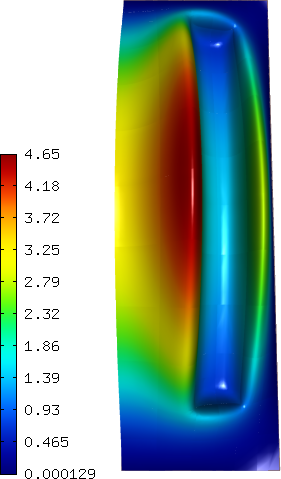
\includegraphics[width=0.5\linewidth]{res/neutronics-4-group/flux4}};
         \node  [right=.8cm of flux4]  (mesh4)  {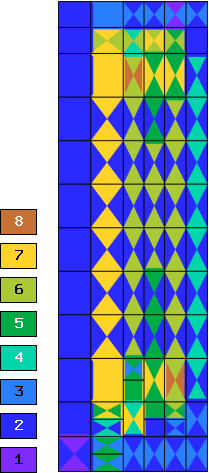
\includegraphics[width=0.37\linewidth]{res/neutronics-4-group/mesh4}};
         \draw
          let
            \p1 = (flux4.south west),
            \p2 = (flux4.south east)
          in
            node [below=.4cm of flux4.south, popis, text width={.9*(\x2-\x1)}] (flux4lbl) {
              $\varphi_{\mathrm{thermal}}$
            };
            
        \draw
          let 
            \p1 = (mesh4.south),
            \p2 = (flux4lbl)
          in
            (\x1,\y2) node [font=\footnotesize, popis] (mesh4lbl) {
              výsledná výpočetní síť
            };
      \end{tikzpicture}
    }
    \begin{minipage}{\linewidth}
      \vspace{0.5cm}
      $\bullet$~Laminární nestlačitelné proudění (NS)
    \end{minipage}\\[1em]
    \noindent\makebox[\textwidth]{ 
      \begin{tikzpicture}[auto]
         \node  at (0,0)               (velocity)  {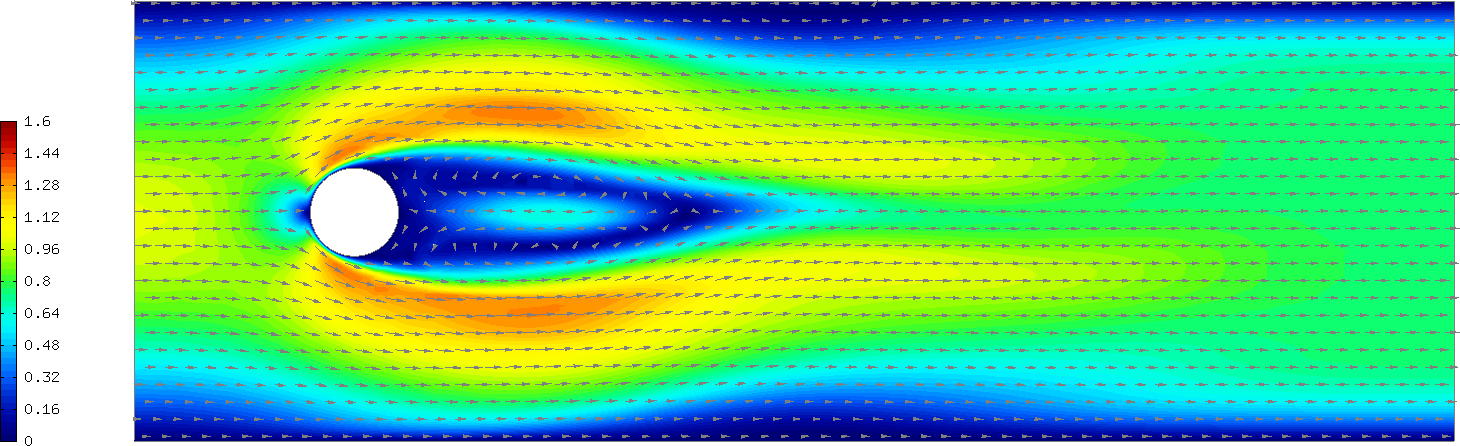
\includegraphics[width=\linewidth]{res/ns/vel}};
         
         \draw
          let
            \p1 = (velocity.south west),
            \p2 = (velocity.south east)
          in
            node [below=.2cm of velocity.south, popis, text width={.9*(\x2-\x1)}] (velocitylbl) {
              rychlostní pole, $t = 20$\;s, spojitá aproximace
            };
         
        \node  [below=.85cm of velocity]  (pressure)  {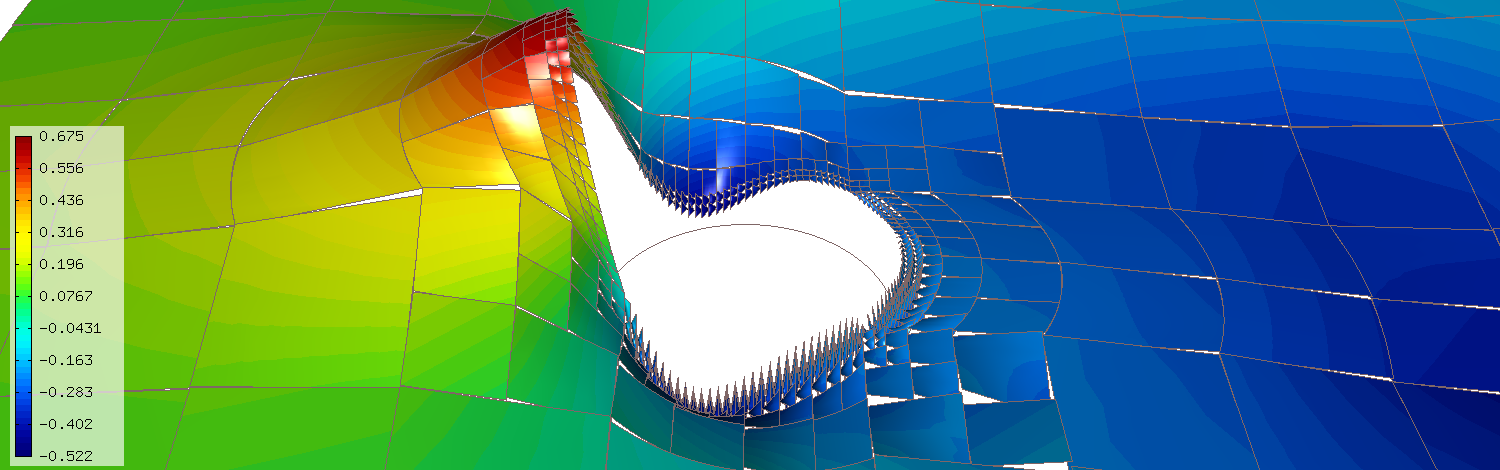
\includegraphics[width=\linewidth]{res/ns/p}};   
        \draw
          let
            \p1 = (pressure.south west),
            \p2 = (pressure.south east)
          in
            node [below=.2cm of pressure.south, popis, text width={.9*(\x2-\x1)}] (pressurelbl) {
              tlakové pole, $t = 20$\;s, nespojitá aproximace
            };
      \end{tikzpicture}
    }
  }
  
%%%%%%%%%%%%%%%%%%%%%%%%%%%%%%%%%%%%%%%%%%%%%%%%%%%%%%%%%%%%%%%%%%%%%%%%%%%%%%
  \headerbox{Neutronika/teplo -- slabá formulace}{name=model,column=0,span=2,below=sdruzene}{
%%%%%%%%%%%%%%%%%%%%%%%%%%%%%%%%%%%%%%%%%%%%%%%%%%%%%%%%%%%%%%%%%%%%%%%%%%%%%%
  %\hspace*{.5em}\begin{minipage}{.95\linewidth}
  \begin{itemize}\compresslist
    %$\bullet$ 
    \item Implicitní Eulerova metoda:~ $\displaystyle\pd{f}{t} \approx \frac{f\it{r}-f\it{r-1}}{\dt}$, ~$f\it{r} \stackrel{\mathrm{ozn.}}{=} f(\bx,t\it{r})$\\[.1em]
    %$\bullet$ 
    \item v čase $t^s$:~
  %\end{minipage}
    $\displaystyle
    \begin{aligned}[t]
      \bF\it{s}(\bY\it{s}) &= \vvec{\bF\it{s}_\flx(\bY\it{s})}{\bF\it{s}_T(\bY\it{s})} = \bO,\quad
      \bY\it{s} = \vvec{\bY\it{s}_\flx}{\bY\it{s}_T},\quad 
      \begin{array}{ll}
        \bY\it{s}_\flx &\mbox{reprezentuje }\ \flx\it{s}\stackrel{\mathrm{ozn.}}{=} \flx(\bx,t^s)\\
        \bY\it{s}_T &\mbox{reprezentuje }\ T\it{s}\stackrel{\mathrm{ozn.}}{=} T(\bx,t^s)
      \end{array}
      \end{aligned}\\[.65em]\hspace*{1em}
    \begin{aligned}
      F_{\flx,i}\it{s}(\bY) &= \vint{\left[\frac{1}{v\dt}\left(\flx\it{s} - \flx\it{s-1}\right)\testN + D\grad \flx\it{s}\grad\testN
                            +\bigl(\Sigma_r(T\it{s})-\nu\Sigma_f\bigr)\flx\it{s}\testN - q_\flx\testN \right]}\\[.15em]
      F_{T,j}\it{s}(\bY) &= \vint{\left[\frac{\rho c_p}{\dt}\left(T\it{s} - T\it{s-1}\right)\testT + k(T\it{s})\grad T\it{s}\grad\testT
                            - \kappa\Sigma_f\flx\it{s}\testT - q_T\testT \right]}
    \end{aligned}
    $\\[.6em]
    s vhodně vybranými funkcemi $\{\testN\}$, $\{\testT\}$.
  \end{itemize}
  \vspace{.1em}
  }
  
%%%%%%%%%%%%%%%%%%%%%%%%%%%%%%%%%%%%%%%%%%%%%%%%%%%%%%%%%%%%%%%%%%%%%%%%%%%%%%
  \headerbox{Řešení ukázkové úlohy\hspace{1.75em} -- adaptace v čase $t_{\mathrm{fin}}=3$\;s:\hspace{7.25em} -- porovnání s přesným řeš.:}{name=reseni,column=0,below=model,span=3}{
%%%%%%%%%%%%%%%%%%%%%%%%%%%%%%%%%%%%%%%%%%%%%%%%%%%%%%%%%%%%%%%%%%%%%%%%%%%%%%
  %\vspace*{-.5em}
  \begin{tikzpicture}[auto]
    \node  at (0,0) (Philbl) {$\flx$: };
    \node  [right=.3cm of Philbl] (Phi1)  {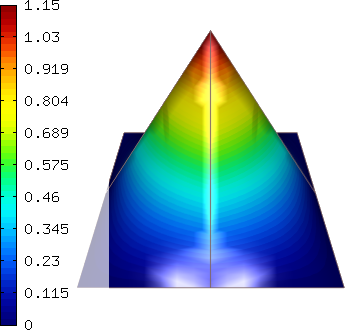
\includegraphics[width=.12\linewidth]{res/neutronics-heat-conduction/Phi1}};
    \node  [below=.11cm of Phi1] (T1)  {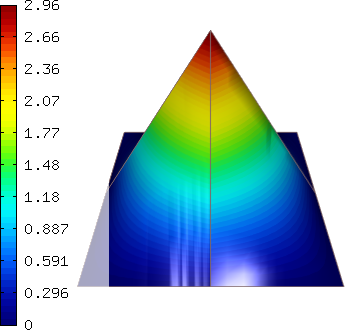
\includegraphics[width=.12\linewidth]{res/neutronics-heat-conduction/T1}};
    \node  [left=.3cm of T1] (Tlbl) {$T$: };
    \node  [right=.75cm of Phi1] (Phi2)  {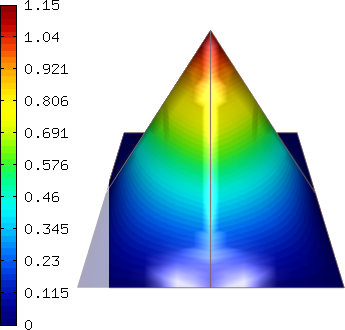
\includegraphics[width=.12\linewidth]{res/neutronics-heat-conduction/Phi2}};
    \node  [below=.13cm of Phi2] (T2)  {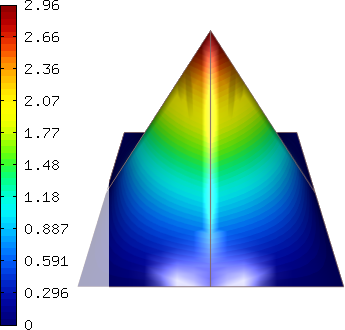
\includegraphics[width=.12\linewidth]{res/neutronics-heat-conduction/T2}};
    \node  [right=.75cm of Phi2] (Phi3)  {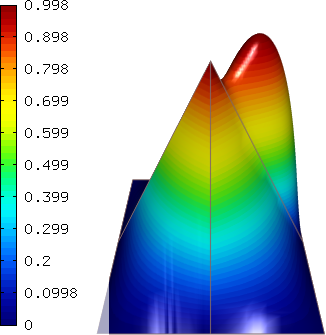
\includegraphics[width=.11\linewidth]{res/neutronics-heat-conduction/Phi3}};
    \node  [below=.15cm of Phi3] (T3)  {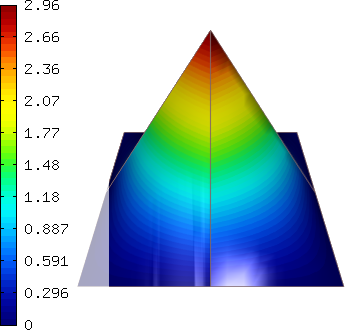
\includegraphics[width=.12\linewidth]{res/neutronics-heat-conduction/T3}};
    \node  [right=.75cm of Phi3] (Phi4)  {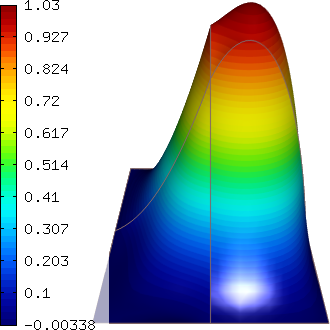
\includegraphics[width=.11\linewidth]{res/neutronics-heat-conduction/Phi4}};
    \node  [below=.15cm of Phi4] (T4)  {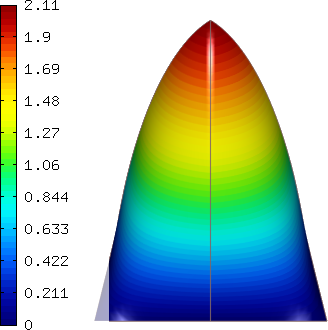
\includegraphics[width=.12\linewidth]{res/neutronics-heat-conduction/T4}};
    \node  [right=.75cm of Phi4] (Phi5)  {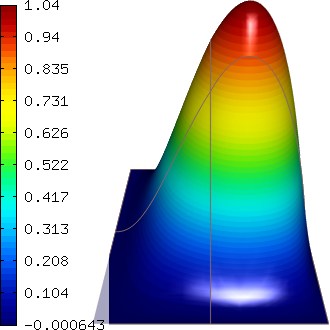
\includegraphics[width=.11\linewidth]{res/neutronics-heat-conduction/Phi5}};
    \node  [below=.15cm of Phi5] (T5)  {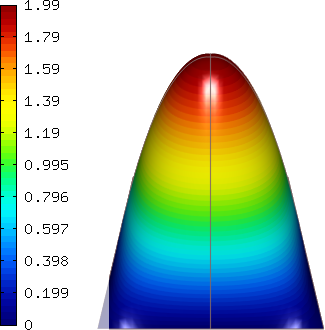
\includegraphics[width=.12\linewidth]{res/neutronics-heat-conduction/T5}};
    \node  [right=1.75cm of Phi5] (PhiErr)  {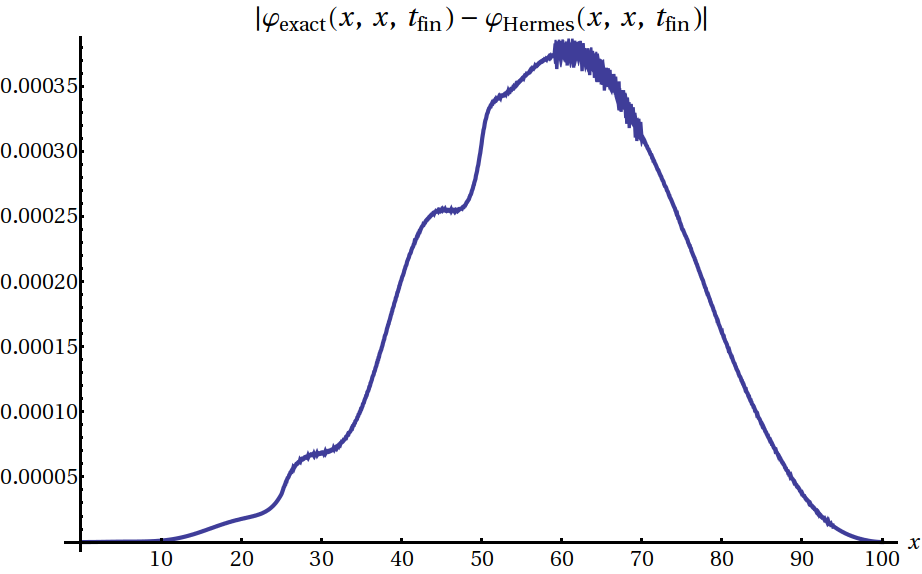
\includegraphics[width=.185\linewidth]{res/neutronics-heat-conduction/PhiErr}};        
    \node  [below=.15cm of PhiErr] (TErr)  {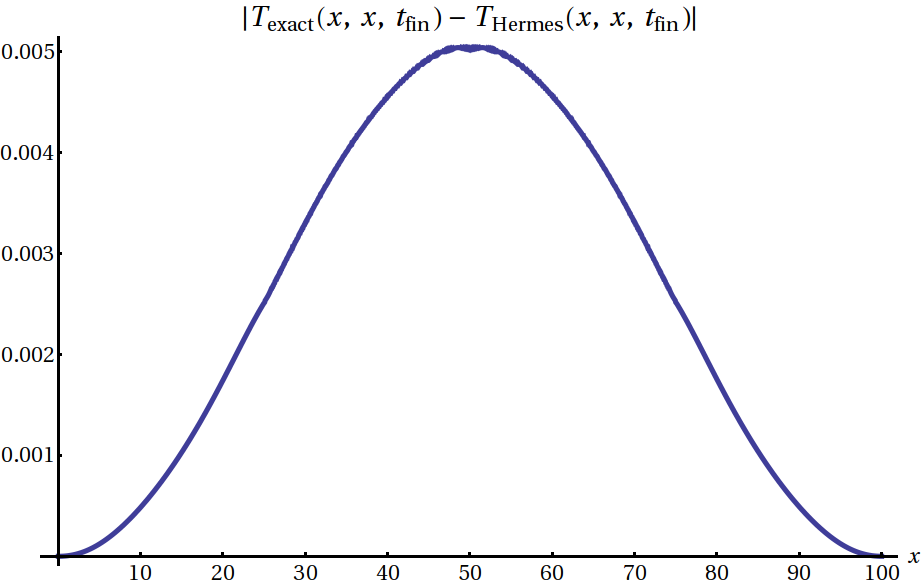
\includegraphics[width=.185\linewidth]{res/neutronics-heat-conduction/TErr}};    
  \end{tikzpicture}
  }  
\end{poster}%
\end{document}
